\section{Minimização de $||\MATRIX{A}\VECTOR{x}-\VECTOR{b}||_{\MATRIX{C}}^2$}

%\index{Problema inverso!Linear}
\index{Minimização do erro quadrático!Linear}%!Função $||\MATRIX{A}\VECTOR{x}-\VECTOR{b}||_{\MATRIX{C}}^2$}

\begin{theorem}\label{theo:minAxbCAxb}
Dados,
um vetor coluna $\VECTOR{x}\in \mathbb{R}^N$, 
um vetor coluna $\VECTOR{b}\in \mathbb{R}^M$,  
uma matriz $\MATRIX{A} \in \mathbb{R}^{M\times N}$, 
uma matriz diagonal $\MATRIX{C} \in \mathbb{R}^{M\times M}$, e 
definida a Eq. (\ref{eq:minAxbCAxb1}),
\begin{equation}\label{eq:minAxbCAxb1}
e(\VECTOR{x})  = ||\MATRIX{A}\VECTOR{x}-\VECTOR{b}||_{\MATRIX{C}}^2.
\end{equation}
Se desejamos ter o valor $\VECTOR{\hat{x}}$ que minimiza o escalar $e(\VECTOR{\hat{x}})$,
devemos usar\footnote{A demostração pode ser vista na Prova \ref{proof:theo:minAxbCAxb}.} a Eq. (\ref{eq:minAxbCAxb2}),
onde o mínimo só existe sim $\MATRIX{A}^{\transpose}\MATRIX{C} \MATRIX{A}$ tem inversa,
\begin{equation}\label{eq:minAxbCAxb2}
\VECTOR{\hat{x}} =
\left[ \MATRIX{A}^{\transpose}\MATRIX{C} \MATRIX{A} \right]^{-1}\MATRIX{A}^{\transpose}\MATRIX{C}\VECTOR{b}.
\end{equation}

\end{theorem}


\begin{corollary}[Vetor perpendicular ao plano 
$\MATRIX{A}\VECTOR{x}$ desde o ponto $\VECTOR{b}$:] 
\label{coro:minAxbCAxb1} ~

\noindent
\begin{minipage}{0.49\textwidth}
\centering
\begin{minipage}{0.93\textwidth}
     \begin{figure}[H]
         \centering
         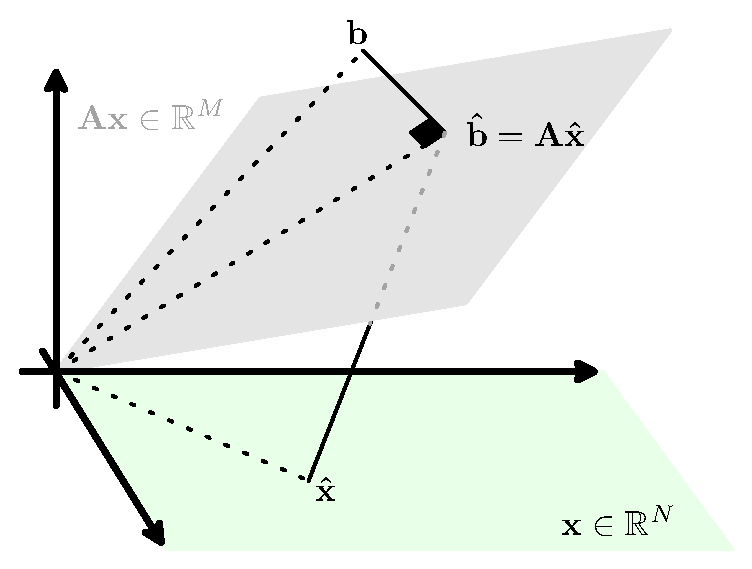
\includegraphics[width=0.9\textwidth]{chapters/minimization-fx/minimo-linear1.eps}
         \caption{Vetor $\VECTOR{d}_p$ perpendicular ao plano 
$\MATRIX{A}\VECTOR{x}$ traçado desde o ponto $\VECTOR{b}$. }
         \label{fig:coro:minAxbCAxb1:a}
     \end{figure}
\end{minipage}
\end{minipage}
\begin{minipage}{0.49\textwidth}
A partir do Teorema \ref{theo:minAxbCAxb}, 
podemos achar um vetor $\VECTOR{d}_p$ perpendicular ao plano $\MATRIX{A}\VECTOR{x}$,
partindo desde o ponto $\VECTOR{b}$, usando a seguinte equação,
\begin{equation}
\VECTOR{d}_p = \left\{\MATRIX{A}\left[ \MATRIX{A}^{\transpose}\MATRIX{A} \right]^{-1}\MATRIX{A}^{\transpose}- \MATRIX{I}\right\}\VECTOR{b},
\end{equation}
onde $I$ é uma matriz identidade.
Podemos ver graficamente o vetor $\VECTOR{d}_p$ na Figura \ref{fig:coro:minAxbCAxb1:a}.
%%
\index{Moore-Penrose!Pseudo-inversa}
\index{Pseudo-inversa!Moore-Penrose}
\begin{tcbattention}
A matriz $\left[ \MATRIX{A}^{\transpose}\MATRIX{A} \right]^{-1}\MATRIX{A}^{\transpose}$
também é chamada de pseudo inversa de Moore-Penrose da matriz $\MATRIX{A}$ \cite[pp. 290]{golub2013matrix}.
\end{tcbattention}
\end{minipage}
\end{corollary}

%%%%%%%%%%%%%%%%%%%%%%%%%%%%%%%%%%%%%%%%%%%%%%%%%%%%%%%%%%%%%%%%%%%%%%%%%%%%%%%%
\subsection{Exemplos de minimização de $||\MATRIX{A}\VECTOR{x}-\VECTOR{b}||_{\MATRIX{C}}^2$}

\begin{example}[Procurando um ponto 
$\VECTOR{\hat{x}}$ que minimize
 $||\MATRIX{A}\VECTOR{x}-\VECTOR{b}||_{\MATRIX{C}}^2$:]
\label{ex:minAxbCAxb1}
Conhecido 
um vetor coluna $\VECTOR{x}\in \mathbb{R}^2$,
as matrizes $\MATRIX{A} \in \mathbb{R}^{3\times 2}$ e $\MATRIX{C} \in \mathbb{R}^{3\times 3}$
e um ponto $\VECTOR{b} \in \mathbb{R}^{3}$,
achar o vetor $\VECTOR{x}$ que minimize $||\MATRIX{A}\VECTOR{x}-\VECTOR{b}||_{\MATRIX{C}}^2$;
sabendo que:
\begin{equation}
\VECTOR{b}=\begin{bmatrix}
1\\
1\\
1
\end{bmatrix},
\qquad 
\MATRIX{A}=\begin{bmatrix}
1 & 0\\
0 & 1\\
1 & 1
\end{bmatrix},
\qquad 
\MATRIX{C}=\begin{bmatrix}
1 & 0 & 0\\
0 & 1 & 0\\
0 & 0 & 1
\end{bmatrix}.
\end{equation}

Podemos ver a resposta a este exemplo na Solução \ref{ex:minAxbCAxb:sol1}.
\end{example}


\begin{SolutionT}[Relativa ao Exemplo \ref{ex:minAxbCAxb1}:]
\label{ex:minAxbCAxb:sol1}
Com todos estes dados e usando a Eq. (\ref{eq:minAxbCAxb1}),
obtemos a superfície $e(\VECTOR{x})$ como mostra a Figura \ref{fig:ex:minAxbCAxb:a}.
Usando a Eq. (\ref{eq:minAxbCAxb2}) sabemos que o ponto $\VECTOR{\hat{x}}=[1\quad 1]^{\transpose}$
minimiza a Eq. (\ref{eq:minAxbCAxb1}), com um $e(\VECTOR{\hat{x}})=0.12$.

Usando o Corolário \ref{coro:minAxbCAxb1}, podemos calcular o vetor $\VECTOR{d}_p=[0.2 \quad 0.2 \quad -0.2]^{\transpose}$,
como mostra o gráfico da Figura \ref{fig:ex:minAxbCAxb:b}.

\begin{figure}[h!]
     \centering
     \begin{subfigure}[b]{0.66\textwidth}
         \centering
         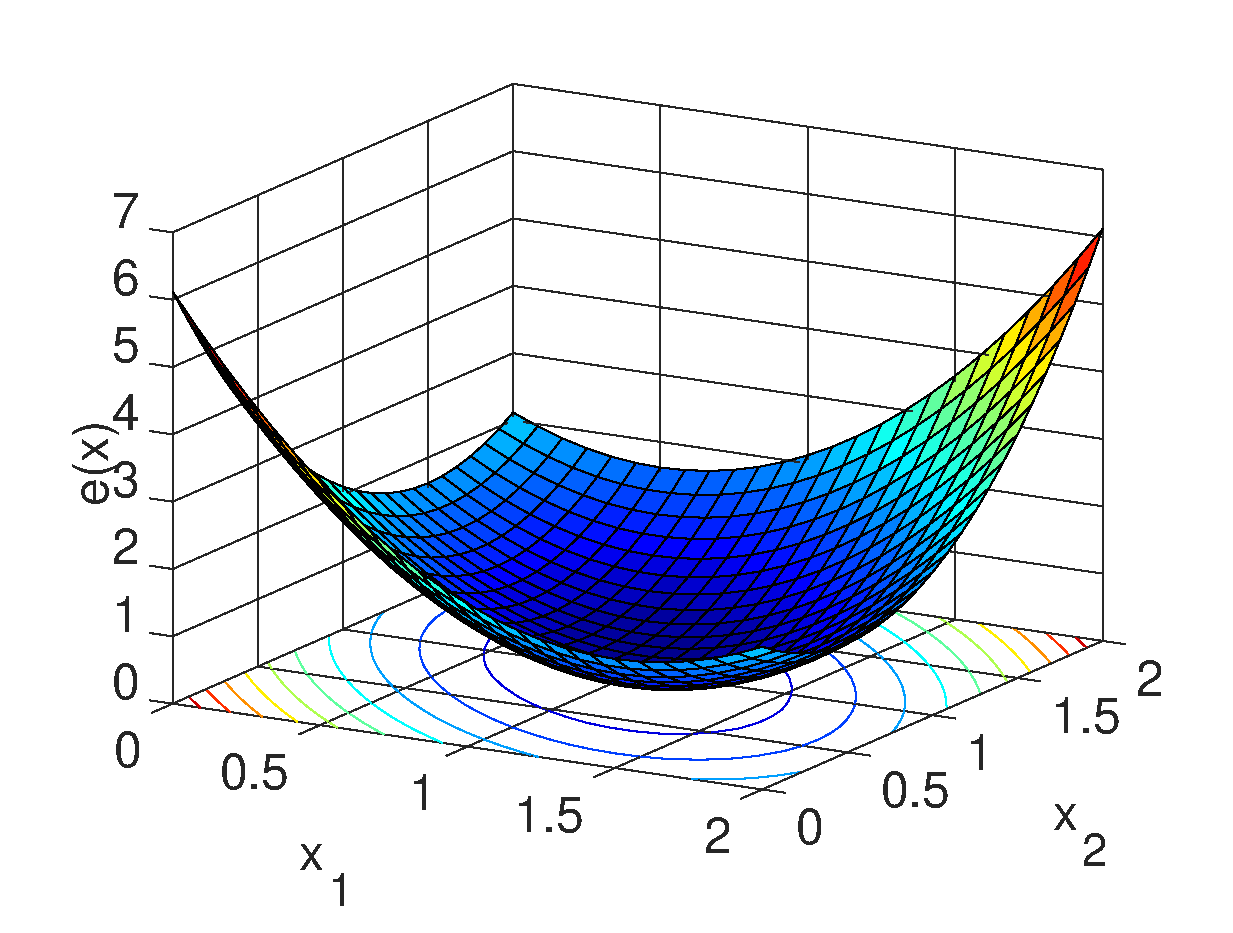
\includegraphics[width=0.98\textwidth]{chapters/minimization-fx/mfiles/ax1/surfcex.eps}
         \caption{Superficie $e(\VECTOR{x})$. }
         \label{fig:ex:minAxbCAxb:a}
     \end{subfigure}
     \hfill
     \begin{subfigure}[b]{0.32\textwidth}
         \centering
         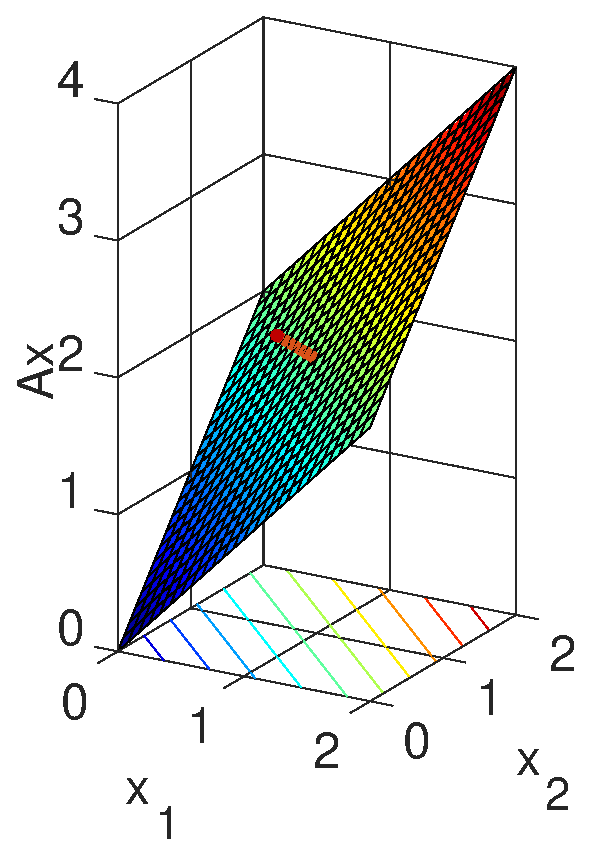
\includegraphics[width=0.98\textwidth]{chapters/minimization-fx/mfiles/ax1/surfcax.eps}
         \caption{Plano $\MATRIX{A}\VECTOR{x}$ e o vetor perpendicular $\VECTOR{b}-\MATRIX{A}\VECTOR{\hat{X}}$.}
         \label{fig:ex:minAxbCAxb:b}
     \end{subfigure}
        \caption{Resposta gráfica do Exemplo \ref{ex:minfxbCfxb3}. }
        \label{fig:ex:minAxbCAxb}
\end{figure}

\end{SolutionT}
